\section{Motivation for Higgs Pair Production}

Couplings of the Higgs boson to heavy vector bosons and heavy fermions
are quickly established after the Higgs boson discovery. However, the
Higgs boson self-coupling is still an open question and an important
probe to check EWSB.

% Super excellent talk by Katharine:
% https://indico.cern.ch/event/1065153/attachments/2351166/4011032/Seminar.pdf

Taylor expansion of the Higgs potential about the minimum after EWSB:
\begin{align*}
  V(h) &= \frac{1}{2} m_{\PH}^2 h^2 + \lambda v h^3 + \frac{1}{4} \lambda h^4 + \dots \\
  m_{\PH} &= \sqrt{2 \lambda v} \approx \SI{125}{\GeV} \\
  \lambda &\approx 0.13 \quad \text{(SM)}
\end{align*}
$h$ is a complex field with the $h^2$-term being the mass term,
$h^3$-term yielding the trilinear coupling, and the $h^4$-term
yielding the quartic coupling. All these terms are directly predicted
by the SM but an experimental probe is still justified to detect
possible deviations from the SM. The self-coupling strength~$\lambda$
can be directly probed in either double Higgs boson production or
triple Higgs boson production (although inaccessible
currently). Indirect probes also exist for example in single Higgs
boson production where the self-coupling contributes at loop-level.

Cross section of HH production is 1000 times smaller than single
Higgs. \todo{Cross section diagram would be nice?}

Motivation:
\begin{description}

\item[Vacuum Stability] The present minimum with a vacuum expectation
  value of $v \approx \si{246}{\GeV}$ might be either a global minimum
  in which case the universe is stable or only a local minimum which
  leads to a metastable universe. In the metastable case, the state of
  the Higgs field could tunnel to a new local or global minimum with a
  smaller vacuum expectation value. Current experimental data cannot
  distinguish whether the universe is stable or
  meta-stable\todo{citation}.

\item[Elektroweak phase transition] In baryogenesis a first order
  electroweak phase transition is needed.

\item[BSM] Radions, 2HDM, Warped extra dimensions, composite Higgs,
  hMSSM, KK Gravitons: Most could decay to pairs of SM Higgs bosons.

\end{description}



\subsection{Search channels for Higgs boson pair production}

\begin{figure}[htbp]
  \centering
  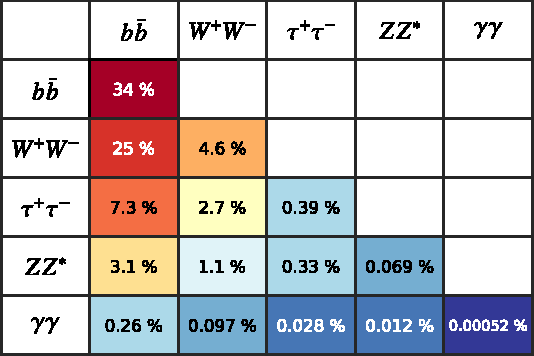
\includegraphics[width=0.45\textwidth]{theory/di_higgs_branching_ratio}
  \caption{Possible final states of decays of pairs of Standard Model
    Higgs bosons. Higgs boson branching ratios are taken
    from~\cite{deFlorian:2016spz} and
    assume~$m_{\PH} = \SI{125.0}{\GeV}$. The decay
    mode~$\PH \ra \Pgluon\Pgluon$ is excluded due to limited
    experimental feasibility.}
  \label{fig:hh_branching_ratios}
\end{figure}

4b: Very large branching ratio but huge multi-jet background.

bbtautau: Can suppress multi-jet background reasonably but large
backgrounds from EW and top.

bbyy: Very clean, but low BR.



Sensitivity vs mass:

bbyy: Low mass sensitivity (due to low threshold photon triggers)

bbtautau: Medium mass sensitivity

bbbb: High mass sensitivity (BR and reduced problems in finding Higgs
candidates due to boost)


\subsection{Review of searches for Higgs boson pair production}

Brief review of previous results / prospects.


\section{Hadron Collider Physics}


Description of the hard scatter event in pp collisions:
\begin{itemize}
\item Collisions of constitutents (partons) of the protons with
  various fractions of momentum of the parent proton.

\item Factorisation approach? Factorise long-distance (soft and
  non-perturbative) and short-distance (hard and perturbative) physics
  at the factorisation scale $\mu_\text{F}$. Long-distance effects are
  factored out into the PDFs while the partonic cross section only
  contains short-distance interactions allowing for perturbative
  expansion in \alphas. The factorisation scale separates partons
  described by the PDF (soft) and the hard scatter process. The
  calculation becomes less dependent on the scale the higher the order
  of the calculation (thus frequently used to estimate uncertainties
  on missing higher orders).

\item The partonic cross section is calculated in a perturbative
  expansion in \alphas up to some order.
\end{itemize}

\begin{align*}
  \sigma_{\Pproton\Pproton \ra \PX}() = \sum_{i,j} \int \mathrm{d}x_1 \mathrm{d}x_2 \, f_i(x_1, \muF^2) f_j(x_1, \muF^2) \, \hat{\sigma}_{i j \ra \PX}(x_1, x_2, \alphas, Q^2 / \muF^2)
\end{align*}
(Ellis, Stirling, Webber)



The inclusive cross section of proton-proton going to \PX is (factorisation approach)
\begin{align*}
  \frac{\mathrm{d}\sigma_{\Pproton\Pproton \ra \PX}}{\mathrm{d}\Omega} = \sum_{i,j} \int \mathrm{d}x_1 \mathrm{d}x_2 \int f_i(x_1) f_j(x_2) \, \mathrm{d}\hat{\sigma}_{i j \ra \PX}(x_1, x_2, \hat{s})
\end{align*}
where $i, j$ indicates the species of parton (i.e.\ gluons, quarks and
anti-quarks), $f_i(x)$ are the corresponding parton density functions,
and $\mathrm{d}\hat{\sigma}(i\,j \ra \PX)$ is the partonic cross
section at a c.m. of $\hat{s} = x_1 x_2 s$.


%%% Local Variables:
%%% mode: latex
%%% TeX-master: "../../phd_thesis"
%%% End:
